\section{Conclusion and future work} \label{sec:conclusion}

In this paper, a brief overview of exploration strategies in both 2D and 3D spaces is given. A modular approach to autonomous decentralized multi-robot exploration and mapping is presented. 
Future research in 2D space should consider decentralized map creation during exploration using a multi-robot system. Given this state-of-the art overview, one research direction can be an extension to the algorithm to cope with a limited communication range of the robots. Moreover, frontier detection and filtering problem combined with exploration is also an interesting research direction.

This paper presents an overview of 3D exploration strategies, as well as a solution for autonomous exploration of 3D environments using a single robot, and without a priori map given.

If we consider 3D exploration, an extension to multi unmanned aerial vehicles (UAVs) system using coordinated exploration strategy can be a significant improvement. Also, if we enable map sharing among robots, we can improve overall behavior of each robot. 

Finally, we would like to take into consideration scenarios in which the robots might fail as well as scenarios with time-varying environments.

To conclude, this work is a stepping stone for new research in coordinated multi-robot exploration algorithms and its decentralization.

\begin{figure}[t!]
	\centering
	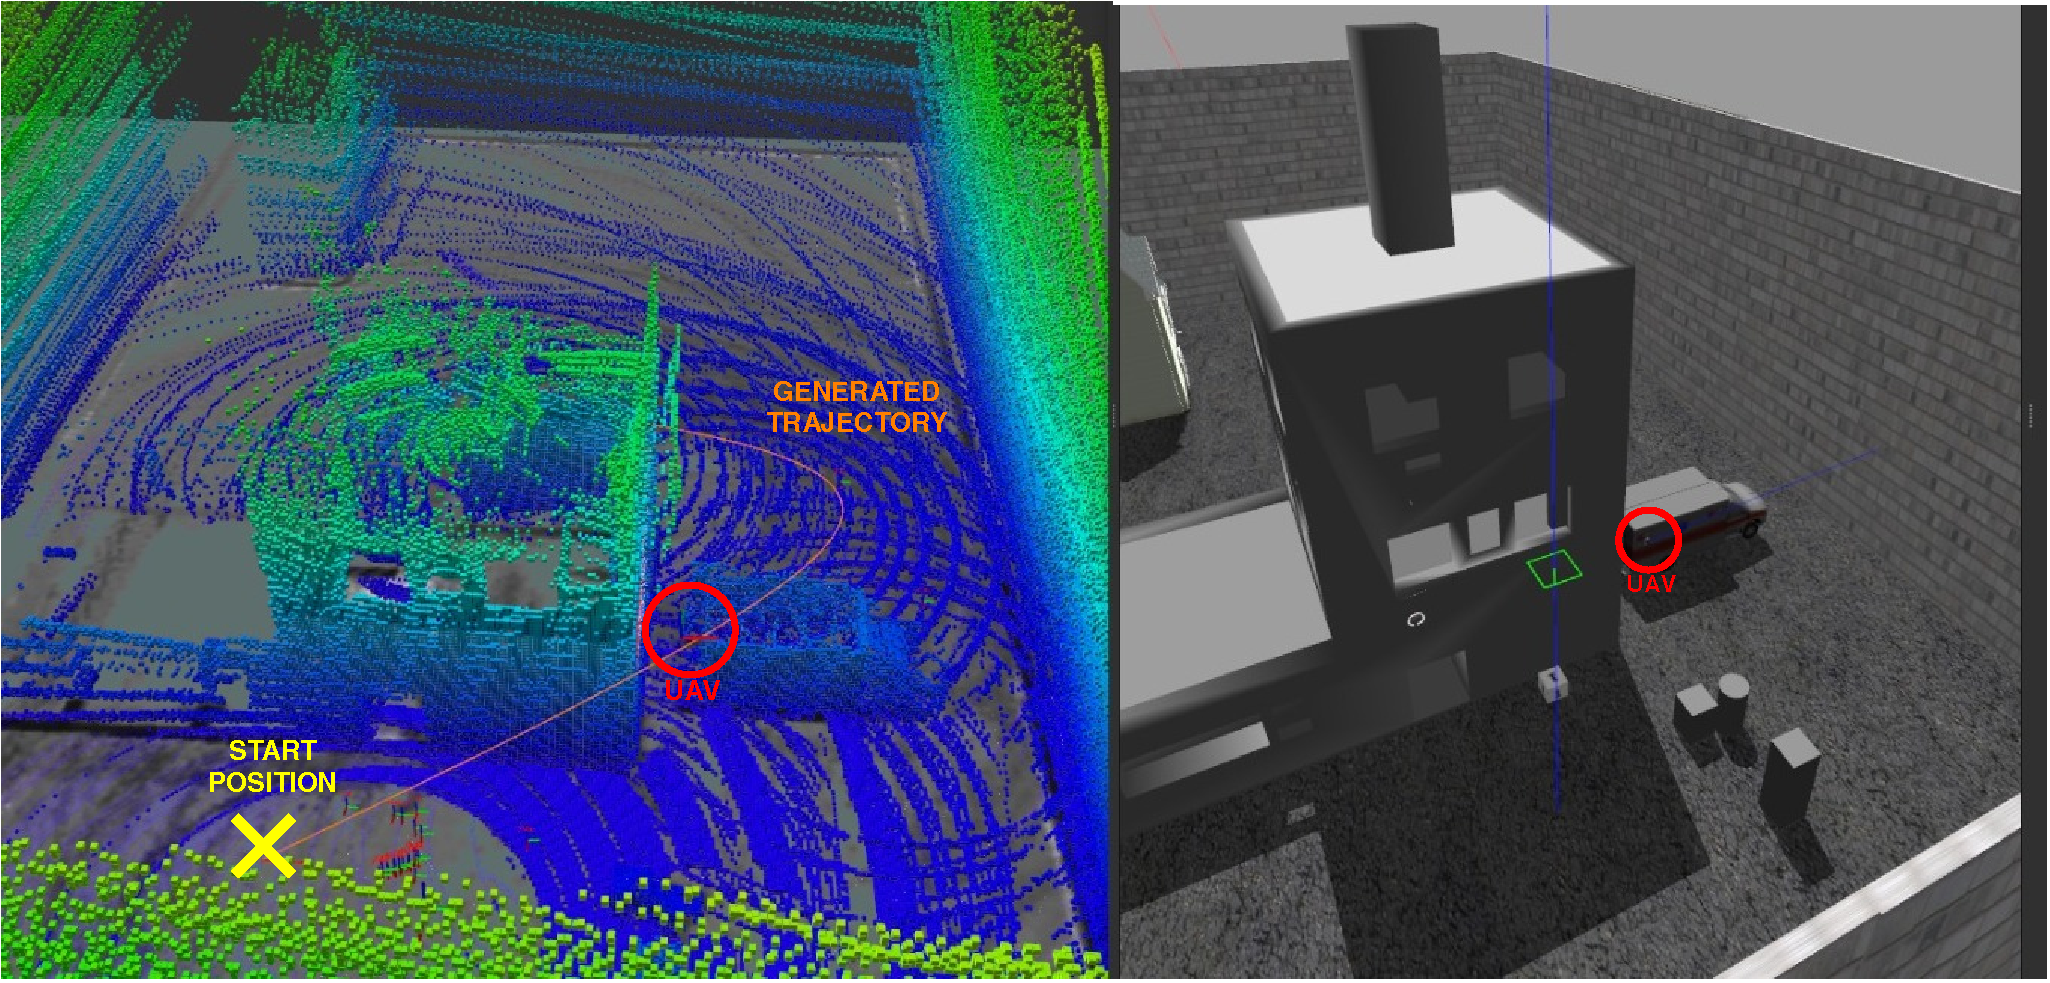
\includegraphics[width=1.0\columnwidth]{./pictures/rviz_gazebo.pdf}	
	\caption{Execution of the generated trajectory.}
	\label{fig:rviz_gazebo}
\end{figure}